\documentclass[UTF8,a4paper,10pt]{ctexart}
\usepackage[left=2.50cm, right=2.50cm, top=2.50cm, bottom=2.50cm]{geometry} %页边距
\CTEXsetup[format={\Large\bfseries}]{section} %设置章标题居左
 
 
%%%%%%%%%%%%%%%%%%%%%%%
% -- text font --
% compile using Xelatex
%%%%%%%%%%%%%%%%%%%%%%%
% -- 中文字体 --
%\setmainfont{Microsoft YaHei}  % 微软雅黑
%\setmainfont{YouYuan}  % 幼圆    
%\setmainfont{NSimSun}  % 新宋体
%\setmainfont{KaiTi}    % 楷体
%\setCJKmainfont{AR PL SungtiL GB}   % 宋体
%\setmainfont{SimHei}   % 黑体
% -- 英文字体 --
%\usepackage{times}
%\usepackage{mathpazo}
%\usepackage{fourier}
%\usepackage{charter}
\usepackage{helvet}
 
\usepackage[colorlinks,linkcolor=black, anchorcolor=green, citecolor=black]{hyperref} 
\usepackage{amsmath, amsfonts, amssymb} % math equations, symbols
\usepackage[english]{babel}
\usepackage{color}      % color content
\usepackage{graphicx}   % import figures
%\usepackage[colorlinks, linkcolor=blue]{url}        % hyperlinks
\usepackage{bm}         % bold type for equations
\usepackage{multirow}
\usepackage{booktabs}
\usepackage{epstopdf}
\usepackage{epsfig}
\usepackage{algorithm}
\usepackage{algorithmic}
\usepackage{tcolorbox}
\usepackage{colortbl}
%\usepackage{float}
\renewcommand{\algorithmicrequire}{ \textbf{Input:}}     % use Input in the format of Algorithm  
\renewcommand{\algorithmicensure}{ \textbf{Initialize:}} % use Initialize in the format of Algorithm  
\renewcommand{\algorithmicreturn}{ \textbf{Output:}}     % use Output in the format of Algorithm   
 



\usepackage{fancyhdr} %设置页眉、页脚
%\pagestyle{fancy}
\lhead{}
\chead{}
%\rhead{\includegraphics[width=1.2cm]{fig/ZJU_BLUE.eps}}
\lfoot{}
\cfoot{}
\rfoot{}
 
%%%%%%%%%%%%%%%%%%%%%%
% 中文映射
%%%%%%%%%%%%%%%%%%%%%



%%%%%%%%%%%%%%%%%%%%%%%
%  设置水印
%%%%%%%%%%%%%%%%%%%%%%%
%\usepackage{draftwatermark}         % 所有页加水印
%\usepackage[firstpage]{draftwatermark} % 只有第一页加水印
% \SetWatermarkText{Water-Mark}           % 设置水印内容
% \SetWatermarkText{\includegraphics{fig/ZJDX-WaterMark.eps}}         % 设置水印logo
% \SetWatermarkLightness{0.9}             % 设置水印透明度 0-1
% \SetWatermarkScale{1}                   % 设置水印大小 0-1    
 
\usepackage{hyperref} %bookmarks
\hypersetup{colorlinks, bookmarks, unicode} %unicode
 
 
 
\title{\textbf{机器翻译开题报告}}
\author{贾栋\; 王坤}
\date{\today}
 
\begin{document}
    \maketitle


\begingroup % start a TeX group
\color{black}% or whatever color you wish to use
\renewcommand{\contentsname}{目录}
\tableofcontents
\newpage
\endgroup   % end of TeX group
 

%\renewcommand{\abstractname}{抽象}
%\begin{abstract}
%这是一篇中文小论文。这个部分用来写摘要。摘要的章标题默认是英文,还没找到改成中文的方法:(
%\end{abstract} 

\section{实验目标}


%\subsection{实验目标}
此次实验的目标是基于现有研究成果,实现一个中英互译的机器翻译引擎,
可以提供中英互译的基本API。利用实验提供的UMCORPUS 数据集以及其他的一些开源数据集(详情见下文)
进行训练。根据 \href{http://nlpprogress.com/english/machine_translation.html}{\color{blue}nlpprocess} 的记录,
目前在机器翻译领域(基于WMT2014数据集)表现最为优秀的模型是 \href{https://arxiv.org/pdf/1808.09381.pdf}{\color{blue}Transformer Big + BT (Edunov et al., 2018)} (英德互译),
\href{https://www.deepl.com/press.html}{\color{blue}DeepL}(英法互译),以及表现同样较为优秀的 \href{https://arxiv.org/abs/1901.10430.pdf}{\color{blue}DynamicConv (Wu et al, 2019)}
等。其中DeepL是商业软件,
  其他两个都有论文发表。实验的基本思路是借鉴这些优秀论文的思想,比较具体的可行性,
  选取其中的一个进行实现。

从机器翻译的基本方法出发,本次实验选取了能够代表三大方法的开源 ML 引擎进行对比。包含但不限于以下模型:
\begin{itemize}

\item[$$$\bullet$] \href{http://www.statmt.org/moses/?n=Moses.Overview}{\color{blue}\underline{Mose}}  基于统计的 

\item[$\bullet$] \href{https://github.com/apertium}{\color{blue}\underline{Apertium}}                基于规则的

\item[$\bullet$] \href{http://thumt.thunlp.org/}{\color{blue}\underline{THUMT}}                     基于神经网络的
\end{itemize}
   
  最终选用\href{https://arxiv.org/pdf/1808.09381.pdf}{\color{blue}Transformer Big + BT (Edunov et al., 2018)} 作为最终实现目标。
  首先需要建立 Transformer 的基本模型,然后此基础上再进行改进。


\section{实验思路}

   从 MT 基于规则的方法,到依赖于大量数据的基于统计的方法,再到基于深度学习的 seq2seq learning。
   机器翻译领域不断涌现着新的思路和方法,并且表现出更优异的性能。从seq2seq的思路出发,机器翻译模型
   通过将一种语言的输入序列转化为另一种语言的输出序列,从而达到翻译的目的。基本的模型由两个 RNN 组成,
   一个encoder,一个decoder。
   

   由于RNN具有保存先前状态的能力,所以可以学习序列化数据的规律。之后在seq2seq的方法的基础之上,提出了attention机制,
   使得模型性能具有了较大提升。之后又提出的 \href{https://arxiv.org/pdf/1808.09381.pdf}{\color{blue}Transformer Big + BT (Edunov et al., 2018)} 
   不再使用RNN作为encoder$以及$decoder,而是全部使用attention。建立了直接的长距离依赖。


   所以现有的基本思路是建立 Transformer 的模型,通过研读有关论文,在此基础上使用 Back-Translation 的方法。
   最终目标是最大近似的再现\href{https://arxiv.org/pdf/1808.09381.pdf}{\color{blue}Transformer Big + BT}的模型。

\section{Seq2seq 模型简介} 
\subsection{背景}

   Seq2seq 模型是机器翻译,对话生成等任务中的经典模型,attention 机制为其提供了较大的性能改进。
   基本的Seq2seq 模型使用的是复杂的RNN或者CNN作为encode,decoder,加上attention机制后为q模型赋予了较强的区分辨别能力。
   而 Transformer 模型完全使用attention机制摒弃了RNN,CNN。建立了更为简单的模型,得到了优异的性能,
   更易并行化,训练时间更少。原始的 Transformer 模型在WMT2014 英德数据集上取得了28.4BLEU的性能。

   之后还有很多基于Transformer模型的改进,本此报告先总结Transformer原始模型的基本思想以及算法。

\subsection{Attention Mechanism }
   \subsubsection{原理}

    Seq2seq 模型解决的主要问题是如何把一个变长的输入$x$映射到一个变长的输出$y​$。基本的结构如下图所示:
    
    \centerline{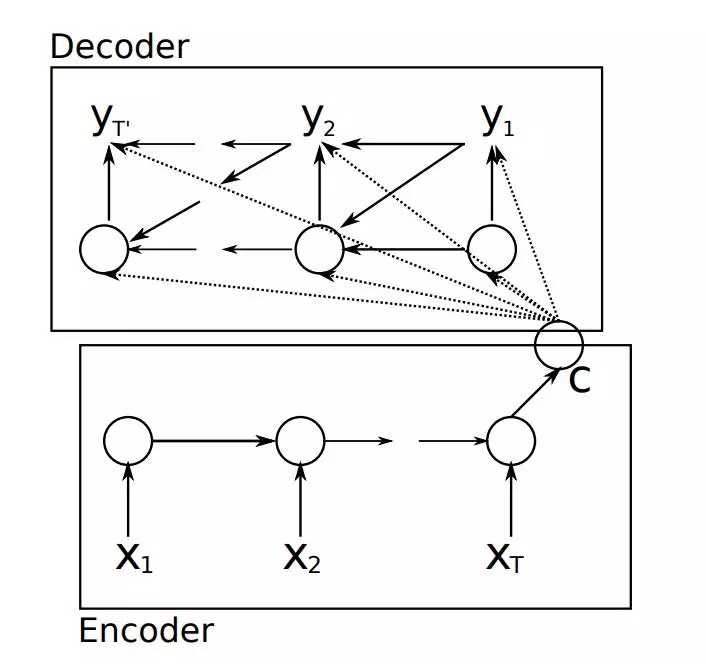
\includegraphics[scale=0.3]{pics/190417-s1.jpg}}
    

    其中Encoder把输入的$T$维向量编码为一个固定长度的隐向量c(或者成为上下文向量context),其作用有二:
    初始化Decoder模型,作为背景向量指导序列中每一步$y_t$的产出。Decoder主要通过每一步的背景向量以及上一步
    的状态$y_{t-1}$得到时刻t的输出$y_t$,直到序列结束(<EOS>)。

    但是基础的Seq2seq模型对于输出序列x缺乏区分度,所以加入的Attention机制,下图是\href{https://arxiv.org/abs/1409.0473}{\color{blue}Bahadanau attention}的示意图:
    
    \centerline{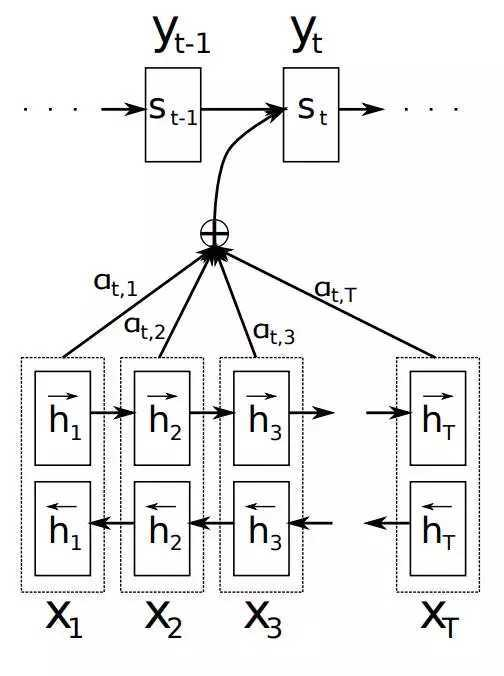
\includegraphics[scale=0.3]{pics/190417-s3.jpg}}
    
    
  
    该模型中定义了一个条件概率:

    \centerline{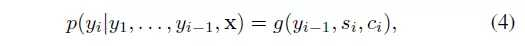
\includegraphics[scale=0.6]{pics/190417-s2.jpg}}
    
    通过attention机制,将输入序列$X =(x_0, x_1, ...,x_T)$ 映射到一个隐层状态$H=(h_0, h_1, ...,h_T)$,再由Decoder将隐层 $H$,映射到输出序列$Y=  (y_0, y_1, ...,y_t)$.这里的精妙之处在于,输出序列Y的每一个元素都与隐层状态H相连,而H又与所有的输入状态存在联系,所以可以直接建立长距离的依赖,发掘更多语义上的关联,从而达到更好的翻译效果。

    \subsection{结构总结}
    
      对于上图文所示的模型,总结如下:
      \begin{itemize}
        \item  使用$h$表示Encoder的隐含状态,$s​$表示Encoder 的隐含状态
         
        \item Encoder将输入$X = (x_0, x_1, ...,x_{T_x})$,通过一个双向LSTM得到两组隐含状态向量$h^{\leftarrow}, h^{\rightarrow}$.然后连接起来得到最终的$H=(h_1,h_2, ...,h_{T_x})$.

        \item 对于Decoder,在时刻$t$时一共有三个输入: $s_{t-1}, y_{t-1}, c_t$,分别代表上时刻的隐含状态、上一时刻的输出、当前步的上下文向量c(即所有Encoder output经过加权得到的一个定长的向量),作为Decoder的上下文。

        \item 有关$c_t$的计算,需要使用softmax作为权重公式,$c_i = \sum_{j=1}^{T_x}a_{ij}h{j}$。其中$a_{ij}$是对应的权值,$h$是Encoder每一步的隐含状态(hidden state, value 或者memory)。i为Decoder step,j为Encoder step。通过这样的权重分配,给与当前上下文相关度较大的状态赋予大的权重,对于Decoder进行解码操作时的影响也就更大,也就是pay more attention

        \item 对于计算$c_i$时使用的权重$a_{ij}$的公式如下:
  $$
              a_{ij} = \frac{exp(e_{ij})}{\sum_{k=1}^{T_x}{exp(e_{ik})}}
  $$
            使用的$e_{ij}$是根据某种度量条件计算得到的$s_{i-1},h_j$的相关程度,计算过程如下:
            \begin{tcolorbox}
               1. 对于$s_{i-1}$做一个线性映射,得到的向量称为query,$q_i$
               \\ 2. 对于$h_i$做一个线性映射,得到的向量称为key, $k_j$
               \\ 3. $e_{ij} = v^T * (q_i + k_j)$; v是一个[d, 1]的向量,$q_i, k_j$ 的维度相同为 d
              \end{tcolorbox}
              以上步骤的线性映射以及v可以通过训练得到,这种方式称为\textbf{加性attention}。

          \item 总结一下,attention就是算一个encoder output的加权和,叫做context;计算方法为,query和key计算相关程度,然后归一化得到alignment,即权重;然后用alignment和memory算加权和,得到的向量就是context。
      \end{itemize}

    \subsection{\textbf{Self Attention}}

   Self Attention 与传统的Attention机制非常的不同:传统的Attention是基于source端和target端的隐含状态(hidden state)
   计算Attention的,得到的结果是源端的每个词与目标端每个词之间的依赖关系。

​    但Self Attention不同,它分别在source端和target端进行,仅与source input或者target input自身相关;
捕捉source端或target端\textbf{自身的词与词之间的依赖关系};然后再把source端的得到的self Attention加入到target端得到的Attention中。

    因此,self Attention Attention比传统的Attention mechanism效果要好,主要原因之一是,传统的Attention机制忽略了源端或目标端句子中词与词之间的依赖关系,
相对比,self Attention可以不仅可以得到源端与目标端词与词之间的依赖关系,同时还可以有效获取源端或目标端自身词与词之间的依赖关系:

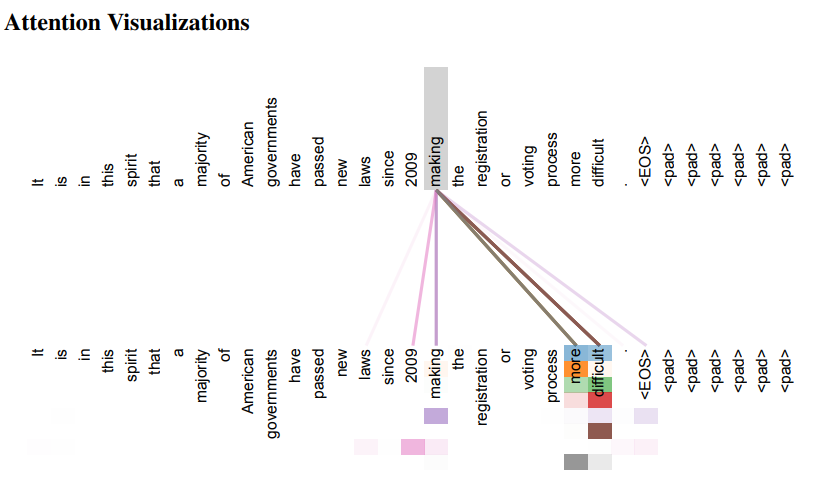
\includegraphics[scale=0.7]{pics/190413-att.png}

Transformer 模型即实现了self-attention.

\section{Transformer}

\subsection{架构}

Trandformer 将传统模型的Encode,Decoder都换为了多个attention。基本示意图如下:

\begin{figure}
\centering
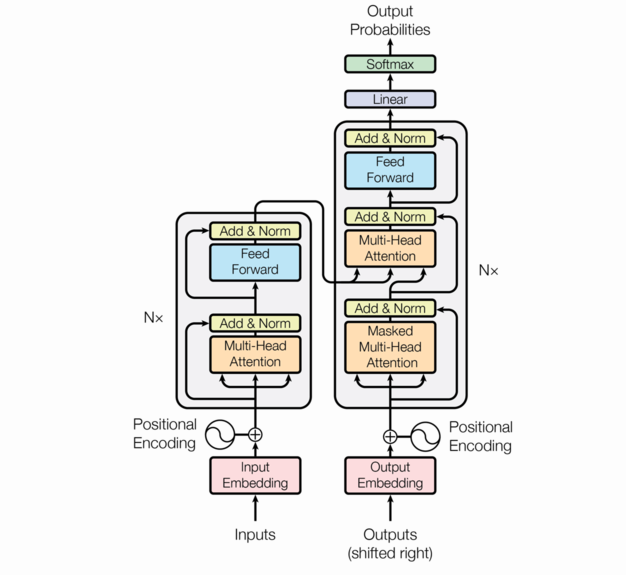
\includegraphics[scale=0.6]{pics/190417-arch.png}
\end{figure}
\begin{itemize}
  \item  左右分别是Encoder和Decoder
  \item Encoder和Decoder的底部是embedding;而embedding又分为两部分:\textbf{input embedding}和\textbf{positional embedding};其中\textbf{input embedding就是seq2seq中的embedding。}
    另一部分是positional embedding,添加该操作是由于transformer中只有attention;而对于attention机制,
    任意一对(query, key)的计算都是完全一样的,不像CNN和RNN,有一个位置或者时序的差异:CNN框住一块区域,随着卷积核移动,
    边缘的少量点会跟着有序变化;RNN更明显了,不同时序的 $h_t$ 和 $s_t$ 不同,而且是随着输入顺序不同(正序,倒序)而不同。
    因此为了体现出时序或者在序列中的位置差异,要对input加入一定的位置信息,即positional embedding。
  \item Encoder 和 Decoder 分别是由N=6 个相同的层叠加得到的。
  \item 对于每一层,Encoder和Decoder的中部分别是两个block,分别输入一个序列、输出一个序列;Encoder的每个block里有两个子层,
    分别是MultiHead Attention和FeedForward Network; Decoder 的block里有三个子层,分别是两个MultiHead Attention和一个FFN。
    这些子网后面都跟了一个add-norm,并且仿照ResNet添加了一个$residual connection$ ,
    对于每一个子层的输出可以形式化表示为$LayerNorm(x + SubLayer(x))$ 也就是子层处理过后的结果加上输入在做正则化处理。
  \item Decoder 的中间的 MultiHead Attention 接受Encoder的输出以及前一个Masked MultiHead Attention 的输出作为输入;
  \item 其中Masked MultiHead Attention是修改过的self-attention, 由于输出的embedding具有一个位置的偏移量,
    使用masking确保了位置i的预测仅取决于小于i的位置处的已知输出。
  \item Decoder最后还有一个Linear和Softmax。
\end{itemize}

\subsection{MultiHead Attention}

这是这篇论文的创新之处,对于原始的attention,就是一个$query$和一组$key$计算相似度,然后对于一组$value$计算加权和$output$。
如果key,query的维度较高,比如均为512维向量,那么就需要在512维的高维空间比较两个向量的相似度。

而MultiHead Attention,则将原本的高维空间通过投影分为多个子空间,例如head\_num = 8,那么就有8个子空间,
相应的value也要分为8个head;然后分别在每一个子空间计算各自query, key的相似度,在分别与value结合。
这样不仅降低了计算成本,便于并行处理,而且可以让attention从多个不同的角度进行结合,这对于NMT工作是很有帮助的。

因为处理翻译任务的source 与target不是一一对应的,而是由多个词共同决定的,进行不同的划分组合后,每一个子空间都可以从各
自关注的角度取组合源语言,从而得到较好的翻译结果。

\subsection{Feed-Forward Network  (FFN)}

基本的前向反馈网络,使用全连接层即可实现。或者使用[1, 1]的卷积实现。使用ReLU作为激活函数。

\centerline{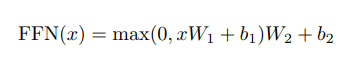
\includegraphics[scale=0.6]{pics/190413-ffn.png}}


\subsection{Positional Embedding}

由于网络中没有使用CNN,RNN,为了使用序列的位置信息,必须添加一些额外的信息确定一个token在序列中的相对或者绝对位置。
文中使用的位置编码公式如下:

\centerline{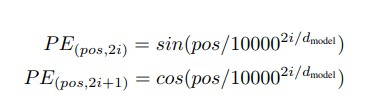
\includegraphics[scale=0.6]{pics/190413-pos.png}}

其中的$pos$是位置,$i$为维度。每一个维度的位置编码为一个正弦曲线,曲线的波长组成了范围在[2$\pi,10000*2\pi$]一个几何级数.
使用这个函数,更容易通过相对位置进行学习,因为对于一个确定的偏差$k$,$PE_{pos+k}$可以使用$PE_{pos}$的线性方程表示。

\section{环境配置}

\subsection{开发环境}
\begin{itemize}
  \item 操作系统: Arch Linux
  \item 编辑器:   vim
  \item 文档:     \LaTeX
\end{itemize}

\subsection{运行环境}

\begin{itemize}
  \item Docker: 18.09.4-ce
  \item docker image: tensorflow/tensorflow:1.12.0-gpu-py3
  \item cuda: 9.0
  \item cudnn: 7.1
  \item tensorflow-1.12.0
  \item keras-2.2.4
  \item numpy-1.15.4
  \item scipy-1.1.0
  \item scikit-learn0.20.0
  \item scikit-image0.12.3
  \item torch-1.0.0
\end{itemize}

\subsection{语料库扩充}

在给定的语料库基础之上,又选取了一些开源的中英平行语料库进行扩充,具体语料库如下:

\centerline{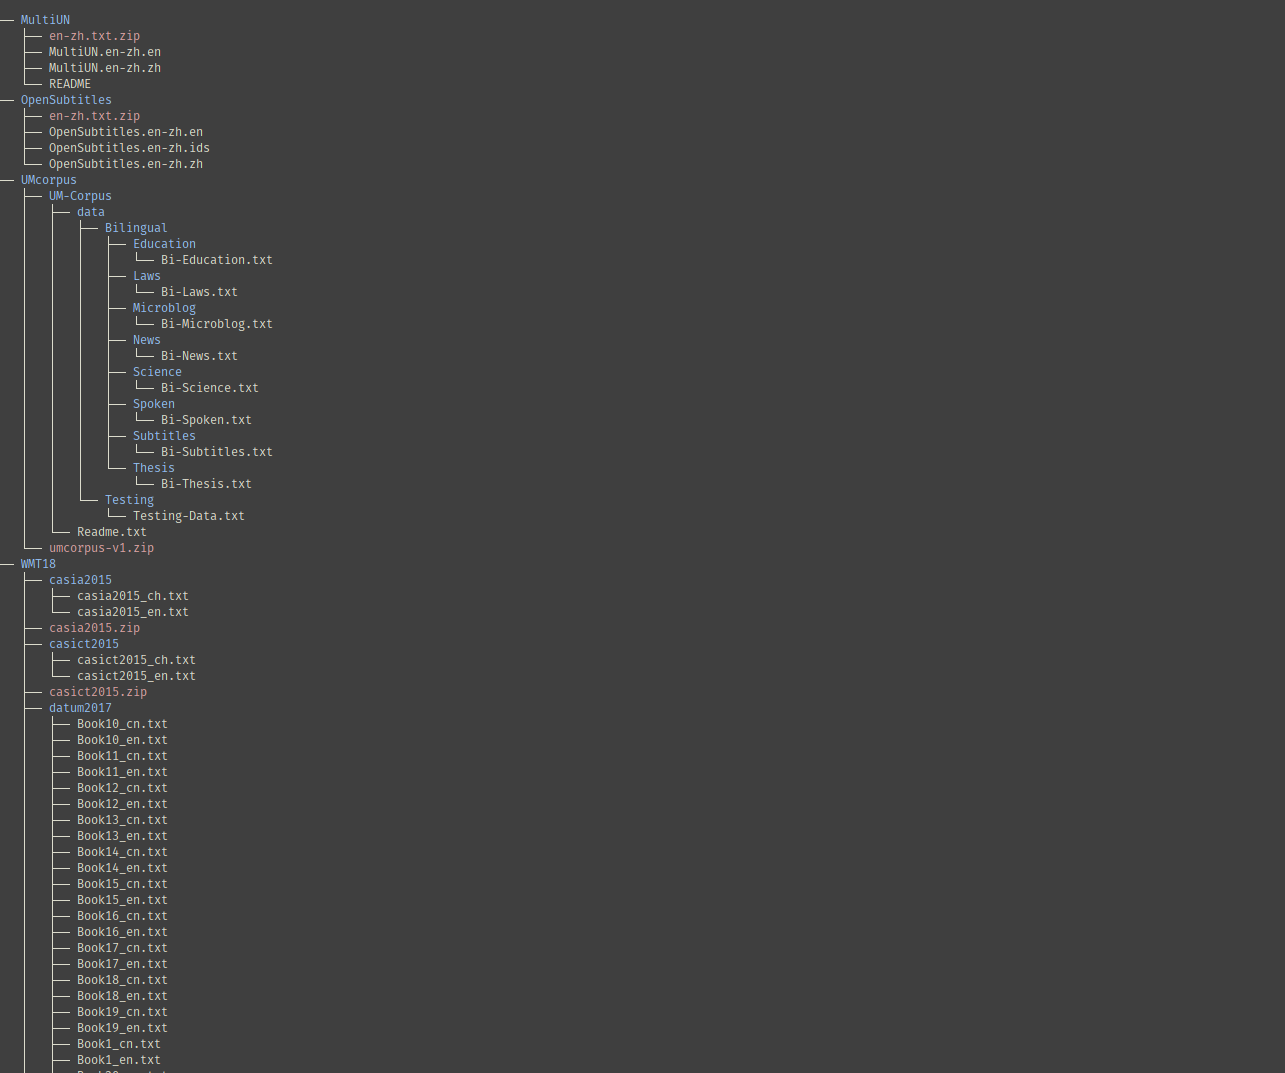
\includegraphics[scale=0.5]{pics/corpus.png})}
\textit{Total: 5.5G}

\section{分工}
\begin{tabular}{ccc}
\hline
姓名& 学号& 任务\\
\hline
贾栋&201600301129 &Transformer 模型的搭建,并在此基础上改进;实验报告的书写\\
王坤&201600301225 &数据的收集与整理;三大开源模型的源码分析,以及模型比对\\
\hline
\end{tabular}

\section{Reference:}

\href{https://arxiv.org/pdf/1409.0473.pdf}{\color{blue}Bahadanau attention}

\href{https://arxiv.org/pdf/1706.03762.pdf}{\color{blue}Attention is all you need}

\href{https://arxiv.org/pdf/1808.09381.pdf}{\color{blue}https://arxiv.org/pdf/1808.09381.pdf}

\href{https://zhuanlan.zhihu.com/p/38485843}{\color{blue}https://zhuanlan.zhihu.com/p/3848584}

\href{https://juejin.im/entry/5a1f9e036fb9a0450671663c}{\color{blue}https://juejin.im/entry/5a1f9e036fb9a0450671663c}

 
\bibliographystyle{plain}
\bibliography{sample}

\end{document}

